%
% File coling08.tex
%
% Contact: R.P.Evans@brighton.ac.uk

\documentclass[11pt]{article}
\usepackage{naaclhlt2009}
\usepackage{times} 
\usepackage{latexsym}
\usepackage[round]{natbib} 
\usepackage{amsmath}
\usepackage{amssymb} 
\usepackage{array} 
\usepackage[pdftex]{graphicx} 
\usepackage{hyperref} 

%% sloppy linebreaks 
%\sloppy 

%% no extra spacing after dots
%\frenchspacing

%% interline spacing
\renewcommand{\baselinestretch}{.967} 

\setlength\titlebox{6.5cm}    % Expanding the titlebox

\title{Multilingual Semantic Role Labelling with Markov Logic}

\author{
Ivan Meza-Ruiz\footnotemark[1]  \qquad Sebastian Riedel\footnotemark[2] 
\footnotemark[3]   \\
\footnotemark[1]  {School of Informatics, University of Edinburgh, UK}\\
\footnotemark[2]  {Department of Computer Science, University of Tokyo, Japan}\\
\footnotemark[3]  {Database Center for Life Science, Research Organization of 
Information and System, Japan}\\
\footnotemark[1]  \tt  I.V.Meza-Ruiz@sms.ed.ac.uk \footnotemark[2] \tt 
sebastian.riedel@gmail.com
}



\date{} 

\begin{document} 



%%% Local Variables: 
%%% mode: latex
%%% TeX-master: "paper"
%%% End: 

\newcommand{\word}{\mathit{word}}
\newcommand{\isArgument}{\mathit{isArgument}}
\newcommand{\sense}{\mathit{sense}}
\newcommand{\lemma}{\mathit{lemma}}
\newcommand{\ppos}{\mathit{ppos}}
\newcommand{\cpos}{\mathit{cpos}}
\newcommand{\role}{\mathit{role}}
\newcommand{\hasRole}{\mathit{hasRole}}
\newcommand{\feat}{\mathit{feat}}
\newcommand{\dep}{\mathit{dep}}
\newcommand{\myframe}{\mathit{frame}}
\newcommand{\predicate}{\mathit{predicate}}
\newcommand{\possibleArg}{\mathit{possibleArg}}

\newcommand{\R}{\mathcal{R}}
\newcommand{\T}{\mathcal{T}}
\newcommand{\bv}{\mathbf{v}}
\newcommand{\score}{s}
\newcommand{\obs}{\x_{o}}
\newcommand{\imp}{\Rightarrow}
\newcommand{\equi}{\Leftrightarrow}
\newcommand{\boldc}{\mathbf{c}}
\newcommand{\boldv}{\mathbf{v}}


\newcommand{\w}{\mathbf{w}}
\newcommand{\Y}{\mathcal{Y}}
\newcommand{\Yvar}{\mathbf{Y}}
\newcommand{\F}{F}
\newcommand{\opti}{\hat{\x}_{h}}
\newcommand{\f}{\mathbf{f}}
\newcommand{\x}{\mathbf{x}}
\newcommand{\y}{\mathbf{y}}
\newcommand{\ybest}{\hat{\y}}
\newcommand{\h}{\mathbf{h}}
\newcommand{\X}{\mathbf{X}}
\newcommand{\D}{\mathcal{D}}
\newcommand{\argmax}[1]{\underset{#1}{\text{arg max}}}
\newcommand{\guess}{\y'}
\newcommand{\Real}{\mathbb{R}}
\newcommand{\Int}{\mathbb{N}}
\newcommand{\bilevel}{\left\langle \Gamma,M\right\rangle }
\newcommand{\vocab}{\text{Vocabulary}}
\newcommand{\reduct}{\text{Reduct}}
\newcommand{\lforall}{\dot{\forall}}
\newcommand{\sscore}{\varsigma_{M}}
\newcommand{\cand}{\text{Cand}}
\newcommand{\unroll}{\text{Unroll}}
\newcommand{\ground}{\text{Ground}}
\newcommand{\mater}{\text{Materialize}}
\newcommand{\inner}{\text{Inner}}
\newcommand{\mapmodel}{\hat{N}}
\newcommand{\prob}{p}
\newcommand{\separate}{\text{Separate}}
\newcommand{\solve}{\text{solve}}
\newcommand{\MAP}{\text{MAP}}
\newcommand{\boldG}{\mathbf{G}}
\newcommand{\round}{\text{Round}}
\newcommand{\fracsolve}{\text{fractional-solve}}
\newcommand{\fractionals}{\text{Fractionals}}
\newcommand{\atoms}{\text{Atoms}}
\newcommand{\aux}{\lambda}
\newcommand{\smokes}{\forall x.\forall y.friends\left(x,y\right)\wedge smokes\left(x\right)\Rightarrow smokes\left(y\right)}
\newcommand{\data}{\mathcal{D}}
\newcommand{\I}{\mathbb{I}}
\newcommand{\Cliques}{\mathcal{C}}
\newcommand{\weightedsmokes}{\forall x.\forall y.\left(friends\left(x,y\right)\wedge smokes\left(x\right)\Rightarrow smokes\left(y\right)\left[w_{smokes}\right]\right)}
\newcommand{\ilpy}{\mathbf{a}}
\newcommand{\powerset}{\mathcal{P}}
\newcommand{\innersmokes}{friends\left(x,y\right)\wedge smokes\left(x\right)\Rightarrow smokes\left(y\right)}
\newcommand{\annasmokes}{smokes\left(Anna\right),friends\left(Anna,Peter\right)}
\newcommand{\finitevocab}{\left\{  \left\{  smokes,friends\right\}  ,\left\{  \right\}  ,\left\{  Anna,Peter\right\}  ,\left\{  x,y\right\}  \right\}  }
\newcommand{\determin}{\text{Deterministic}}
\newcommand{\nondeter}{\text{Nondeterministic}}


\maketitle
\begin{abstract}
This paper presents our system for the CoNLL 2009 Shared
Task on Syntactic and Semantic Dependencies in Multiple
Languages \citep{CoNLL-2009-ST}. In this work we focus only
on the Semantic Role Labelling (SRL) task. We use Markov Logic to define a joint SRL model and achieve
the third best average performance in the closed Track for SRLOnly systems and 
the sixth including for both SRLOnly and Joint systems.
\end{abstract}
\section{Markov Logic} \label{sec:markovlogic}

%IV: I love this paragraph! Not, really, no joke! I have read it so many times,
%I can almost recite it. It can be rapped.
Markov Logic \citep[ML, ][]{richardson05markov} is a Statistical Relational Learning language based on First Order Logic and Markov Networks. It can be seen as a formalism that extends First Order Logic to allow formulae that can be violated
with some penalty. From an alternative point of view, it is an expressive
template language that uses First Order Logic formulae to instantiate
Markov Networks of repetitive structure. 

Let us describe ML by considering the predicate identification task. In ML we can model this task by first introducing a set of logical predicates\footnote{In the cases were is not obvious whether we refer to SRL or ML predicates we add the prefix SRL or ML, respectively.} such as \emph{isPredicate(Token)} or \emph{word(Token,Word)}. Then we specify a set of weighted first order formulae that define a distribution over sets of ground atoms of these predicates (or so-called \emph{possible worlds}). 

Ideally, the distribution we define with these weighted formulae assigns high probability to possible worlds where SRL predicates are correctly identified and a low probability to worlds where this is not the case. For example, a suitable set of weighted formulae would assign a high probability to the world\footnote{``Haag plays Elianti'' is a segment of a sentence in the training corpus.}
% SR: made words more distinct from predicates/variables (suggested by Ewan in my thesis)
\begin{eqnarray*}
 &\{ word\left(1,\text{Haag}\right),word(2,\text{plays}),\\
 & word(3,\text{Elianti}),isPredicate(2) \}& \end{eqnarray*}
and a low one to
\begin{eqnarray*}
& \{ word\left(1,\text{Haag}\right),word(2,\text{plays}),\\
 & word(3,\text{Elianti}),isPredicate(3) \} &\end{eqnarray*}
% This is the line refered by the reviewer 1 in  point 6.
% SR: Okay, rewrite to get rid of akward indices.
In Markov Logic a set of weighted formulae is called a \emph{Markov Logic Network}~(MLN). Formally speaking, an MLN $M$ is a set of pairs $\left(\phi,w\right)$ where $\phi$ is a first order formula and $w$ a real weight. $M$ assigns the probability
\begin{equation}
\prob\left(\y\right)=\frac{1}{Z}\exp\left(
\sum_{\left(\phi,w\right)\in M} w
\sum_{\boldc\in C^{\phi}}f_{\boldc}^{\phi}\left(\y\right)
\right)
\label{eq:prob}
\end{equation}
% SR: a nice version
to the possible world $\y$.  Here $C^{\phi}$ is the set of all possible
bindings of the free variables in $\phi$ with the constants of our
domain. $f_{\boldc}^{\phi}$ is a feature function that returns 1
if in the possible world $\y$ the \emph{ground formula} we get by
replacing the free variables in $\phi$ by the constants in $\boldc$
is true and 0 otherwise. $Z$ is a normalisation constant. Note that
this distribution corresponds to a Markov Network (the so-called \emph{Ground
Markov Network}) where nodes represent ground atoms and factors represent
ground formulae.


% Here $f_{\boldc}^{\phi}$ is a feature
% function that returns 1 if in the possible world $\y$ the \emph{ground
% formula} we get by replacing the free variables in $\phi$ by the constants
% in $\boldc$ is true and 0 otherwise. $C^{n_{\phi}}$ is the set
% of all tuples of constants we can replace the free variables in $\phi$
% with. $Z$ is a normalisation constant. Note that this distribution corresponds to a Markov Network (the so-called \emph{Ground Markov Network}) where nodes represent ground atoms and factors represent ground formulae.

For example, if $M$ contains the formula $\phi$ \[
word\left(x,\text{take}\right)\Rightarrow isPredicate\left(x\right)\]
then its corresponding log-linear model has, among others, a feature 
$f_{t1}^{\phi}$ for which $x$ in $\phi$ has been replaced by the constant $t_1$ and that returns 1 if \[
word\left(1,\text{take}\right)\Rightarrow isPredicate\left(1\right)\]
is true in $\y$ and 0 otherwise.

We will refer predicates such as \emph{word} as \emph{observed} because they are known in advance. In contrast, \emph{isPredicate} is \emph{hidden} because we need to infer it at test time.




\section{Model} \label{sec:model} 


% To model the SRL as a MLN we define a set predicates to express our knowledge about the words of a sentences and the semantic relations. For example, the predicate \emph{lemma(p,l)} specifies the lemma $l$ for the word in the possition $p$. We say a predicate is grounded when it is in terms of atoms. Using our previous example, a grounded instance is \emph{lemma(4,play)} which means the lemma for the word in the fourth possition is \emph{play}. In ML, there are two types of predicates: observed and hidden. The observed predicates represent the knowledge we are certain about and the hidden represent the knowledge we are interested to know about. In the SRL task, we are interested in the predicates which represent the semantic relations. 

We define five hidden predicates for the three stages of the task. %Figure \ref{fig:achitecture} illustrates these predicates and the stage they belong to. 
For predicate identification, we use the predicates \emph{isPredicate} and \emph{sense}. \emph{isPredicate(p)} indicates that the word in the position $p$ is an SRL predicate while \emph{sense(p,e)} signals that predicate in position $p$ has the sense $e$. %\footnote{The sense corresponds to the label after the  ``.'' symbol in a roleset.}. 

For argument identification, we use the predicates \emph{isArgument} and \emph{hasRole}. The atom \emph{isArgument(a)} signals that the word in the position $a$ is a SRL argument of some (unspecified) SRL predicate while \emph{hasRole(p,a)} indicates that the token at position $a$ is an argument of the predicate in position $p$. 

Finally, for the argument classification stage we define the predicate
\emph{role}. Here \emph{role(p,a,r)} corresponds to the decision that the
argument in the position $a$ has the role $r$ with respect to the predicate in
the position $p$.

% There is a potential problem of coupling the predicates. For instance, the predicate $hasRole(p,a)$ could be true, but there is not guaranty that the predicate $predicate(p)$ is. This situation would lead to arguments without SRL predicates. In the following, subsections we explain how we can constrain these two predicates to be couple using the FOL formulae of the MLN model. Aditionally, we show how we can relate our knowledge from the words with the predicates for the SRL task.


% \begin{figure}
% \begin{center}
%     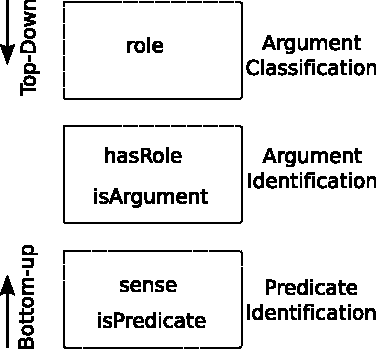
\includegraphics[scale=.70]{TaskArchitecture}
% \end{center}
% \caption{MLN hidden predicates divided in stages}
% \label{fig:achitecture}
% \end{figure}



\subsection{Local formulae}\label{sec:local} 
 

A formula is local if its groundings relate any number of observed ground atoms 
to exactly one hidden ground atom.  For example, a grounding of the local 
formula \[plemma(p,+l_1) \wedge plemma(a,+l_2) \Rightarrow hasRole(p,a)\]
connects a hidden \emph{hasRole/2} ground atom to two observed \emph{lemma/2} 
ground atoms. This formula can be interpreted as the feature for the predicate 
and argument lemmas in the argument identification stage of a pipeline SRL 
system.
Note that the ``+'' prefix signals that there is a different weight for each 
possible pair of lemmas $(l_1,l_2)$.

We divide our local formulae into four sets, one for each hidden predicate.  For 
instance, the set for \emph{argument/1} only contains formulae which hidden 
predicate is \emph{argument/1}. 

The sets for \emph{argument/1} and \emph{sense/2} predicates have similar 
formulae since each predicate only involves one token at time: the SRL argument 
or the SRL predicate. The formulae in this sets are defined using only 
\emph{token} or \emph{extended} observed predicates. There are two differences 
among these two sets.  First, the \emph{argument/1} formulae are condition by
the \emph{possibleArg/1} predicate while sense are condition by 
\emph{predicate/1} predicate. For instance consider the \emph{argument/1} 
formula for the orthography: \[word(a,+w) \land possArgument(a) \land 
argument(a)\], and the contrast for the \emph{sense/2} predicate: \[word(p,+w) 
\land predicate(p) \land sense(p,+s)\]. This means we only apply the 
\emph{argument/1} formulae if the token is a potential SRL argument, and we 
only the \emph{sense/2} formulae if the token is a SRL predicate. The second 
difference is in the arity of the weights. \emph{sense/2} weights are larger by 
one than \emph{argument/2}. This is because their weights include the sense 
label as a part of its indexes. For the orthography formulae, the index for the
first formula is $(+w)$, which is the orthography, while in the second formula 
has as indexes $(+w,+s)$, which is the orthography and the sense label.

These is a summary of the formulae for the \emph{argument/1} and 
\emph{sense/2} sets:
\begin{itemize}\addtolength{\itemsep}{-0.5\baselineskip}
    \item Orthography of the token.
    \item Lemma of a token in a window of $-2 \cdots 2$ tokens.
    \item POS tag of a token in a window of $-2 \cdots 2$ tokens.
    \item Coarse POS tag for the token.
    \item Coarse POS of the two previous and two following tokens.
    \item Dependency relation of the parent and children of a token.
    \item POS tag of children or parent of a token.
    \item POS tag of children or grandchildren and POS tag of token.
    \item POS tag of parent or grandparent and POS tag of token.
    \item Subcategorisation frame of token.
\end{itemize}

The formulae in \emph{hasRole/2} and \emph{role/3} sets are condition both by 
the predicates \emph{possibleArg/1} and \emph{predicate/1} since both try 
to establish a relation between SRL predicate and argument. For these predicate 
we use \emph{toeken}, \emph{extended} and \emph{path} predicates.

This is the summary for the formulae for the \emph{hasRole/2} set:
\begin{itemize}\addtolength{\itemsep}{-0.5\baselineskip}
    \item Lemma of predicate and argument.
    \item POS tags of predicate and argument.
    \item POS tag of predicate and POS tags of argument in a window $-1,+1$.
    \item POS tag predicate and lemma argument.
    \item Lemma predicate and POS tag argument.
    \item Coarse POS tags for predicate and argument in a window $-1,+1$.
    \item POS tag argument and POS tag of children of argument.
    \item POS tag argument and lemma  of children of argument.
    \item Dependency relation with parent for predicate and argument.
    \item Path distance between predicate and argument.
    \item Path and frame of predicate and argument in combination with voice and 
        lemma.
\end{itemize}

This is the summary for the formulae for the \emph{role/3} set:
\begin{itemize}\addtolength{\itemsep}{-0.5\baselineskip}
    \item Lemma of predicate and argument.
    \item POS tag predicate and lemma argument.
    \item POS tag argument and POS tag of children of argument.
    \item POS tag argument and lemma  of children of argument.
    \item Dependency relation with parent for predicate and argument.
    \item Path and frame distance between predicate and argument.
    \item Path and frame of predicate and argument in combination with voice and 
        lemma.
    \item Path of predicate and argument in combination with lemma, POS tag, 
        coarse POS tag.
\end{itemize}

Note that these lists does not mention the feature information. This is because 
this information was not available for each language therefore we  group the 
formulae which contains this predicate into another a set we called 
\emph{feature} formulae. This is the summary of these formulae:
\begin{itemize}\addtolength{\itemsep}{-0.5\baselineskip}
    \item Feature-value pair of the token for \emph{sense/2}.
    \item Feature-value pair of the token for \emph{argument/1}.
    \item Feature-value pair for similar features of the predicate and argument 
        for \emph{hasRole/2}.
    \item Feature-value pair for similar features of the predicate and argument 
        for \emph{role/3}.
\end{itemize}

Additionally, we define a set of language specific formulae. They are aimed to 
capture the relations between argument and its siblings for the \emph{hasRole/2} 
and \emph{role/3} predicates.  In particular, these formulae was beneficial for 
the Japanese language.  This is a summary of such formulae which we called 
\emph{argument siblings}:
\begin{itemize}\addtolength{\itemsep}{-0.5\baselineskip}
    \item POS argument and POS of sibling.
    \item POS argument and lemma sibling.
\end{itemize}

With these set of formulae we can build a specific ML model for a language in 
the share task. Table \ref{tb:diff} shows the difference between languages. We 
omit the \emph{argument/1}, \emph{hasRole/2} and \emph{role/3} because they 
are present for all languages. The \emph{feature} set corresponds to the FEAT 
column provided in the corpus.  The presence of this set is determined by the 
availability of this information in the corpus.  The presence of the 
\emph{sense/2} set is determined by the labelling of senses in the corpora.  
Finally, the formulae for the \emph{argument siblings} was implemented for the 
Japanese during development. 

\begin{table}
\begin{center}
\small
\begin{tabular}{|l|c|c|c|}\hline
    Set             & Feature   & \emph{sense/2}  & Argument \\
                &            &        & siblings  \\\hline\hline
Catalan         &   Yes      &  Yes   &  No  \\
Chinese         &   No       &  Yes   &  No  \\
Czech           &   Yes      &  No    &  No  \\
English         &   No       &  Yes   &  No  \\
German          &   Yes      &  Yes   &  No  \\
Japanese        &   Yes      &  No    &  Yes \\
Spanish         &   Yes      &  Yes   &  No  \\
\hline
\end{tabular}
\caption{Different of formulae between the languages.}
\label{tbl:diff}
\normalsize
\end{center}
\end{table}

A more detail description of the formulae can be found in our MLN model files.  
\footnote{\url{http://thebeast.googlecode.com/svn/mlns/conll09}} They can be 
used both as a reference and as input to our Markov Logic 
Engine\footnote{\url{http://thebeast.googlecode.com}}, and thus allow the reader 
to easily reproduce our results.




\subsection{Global formulae}

%%% Local Variables: 
%%% mode: latex
%%% TeX-master: "paper"
%%% End: 

\emph{Global} formulae relate several hidden ground atoms. We use them for two purposes: to capture some of our intuition about the task and to ensure consistency between the decisions of all SRL stages. We will refer to formulae that serve the first purpose as \emph{structural constraints}. 

% They aim to capture the relations between the hidden predicates, and ultimately of the stages of the SRL task. There are two types of global formulae: \emph{hard formulae} and \emph{soft formulae}. The hard formulae imposes constraints on the structure of the predicates. We can use hard formulae to solve the problem of coupling predicates.
For example, a structural constraint is given by the (deterministic) formula
\[role(p,a,r) \Rightarrow hasRole(p,a)\]
which ensures that whenever the argument $a$ is given a label $r$ with respect to the predicate $p$ this argument must be an argument of $a$ denoted by \emph{hasRole(p,a)}. Note that this formula by itself models the traditional argument identification and classification pipeline: it is possible to not assign a role $r$ to an predicate-argument pair $(p,a)$ proposed by the identification stage; however, it is impossible to assign a role $r$ to token pairs $(p,a)$ that have not been proposed as potential arguments.

One example of another class of structural constraints is 
\[
isPredicate(p)\Rightarrow\exists a.hasRole(p,a)
\]
which, by itself, models a top down pipeline. Here the argument classification stage can assign roles to tokens that are have not been proposed by the argument identification stage. However, it must assign a label to any token pair the previous stage proposes. 
%IV
Figure \ref{fig:global2} ilustrate the structural formulae we use. Notice, that each formulae, represented by the lines, join two hidden predicates.

The formulae we use to ensure consistency between the remaining hidden predicates are omitted for brevity as they are very similar to the bottom-up and top-down formulae we presented above.

For the SRL predicates that perform a labelling task (\emph{role} and \emph{sense}) we also need a structural constraint that ensures that not more than one label is assigned. For instance,
\[
(role(p,a,r_1) \wedge r_1 \neq r_2 \Rightarrow \neg role(p,a,r_2)  )
\]
forbids two different semantic roles for a pair of words. 

% thatrequires that for each \emph{hasRole} predicate there must be a SRL predicate in the postions $p$. This formula help us to relate two of the hidden predicates. The efect of the formula is similar to the bottom-up strategy where after identifing the the arguments of these are classified.

The global formulae that capture our intuition about the task itself can be further divided into two classes. The first one uses deterministic or \emph{hard} constraints such as
\begin{eqnarray*}
 &role\left(p,a_{1},r\right)\wedge \neg mod\left(r\right)\wedge a_{1}\neq a_{2}  \Rightarrow\\
  & \neg role\left(p,a_{2},r\right)
\end{eqnarray*}
which forbids cases where distinct arguments of a predicate have the same role unless the role describes a modifier.
%In this case we constrain to one semantic role to the words identify as proper arguments by the Palmer's heuristics. % ??

The second class of global formulae is \emph{soft} or nondeterministic. For instance, the formula  
\begin{eqnarray*}
  & lemma(p,!l) \wedge ppos(a,!p) \wedge hasRole(p,a)  \Rightarrow \\
  & sense(p,!f) 
\end{eqnarray*}
is a soft global formula. It captures the relation between the \emph{hasRole} and \emph{sense} hidden predicates, together with the lemma of the SRL predicate and the POS tag of the argument. Figure \ref{fig:global2} is a graphical model representing the grounded version of this formula. %This formula does not imposes a structural constrain, but rather the link between the sense of the SRL predicate and its arguments.
%Why would this help?

\begin{figure}
\begin{center}
   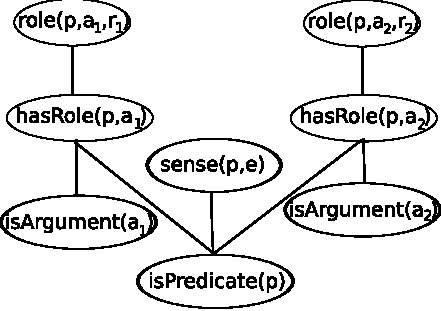
\includegraphics[scale=.70]{GlobalFormula2}
\end{center}
\caption{Factor graph for example of global formula}
\label{fig:global2}
\end{figure}






% Finally, to our last group of rules belongs the soft formulae and hard constrains with extra linguistic knowledge. Figure \ref{fig:global2} shows an example of soft formulae. An example, of hard constriain which uses extra linguistic knowledge is:
% \begin{eqnarray*}
%  & role\left(p,a_{1},r\right)\wedge arg\left(r\right)\wedge a_{1}\neq a_{2} & \Rightarrow\\
%   & \neg role\left(p,a_{2},r\right)
% \end{eqnarray*}
% In this case we constrain to one semantic role to the words identify as proper arguments by the Palmer's heuristics. % ??
%
%We have slit our global formulae into four groups. The first, are hard constrains which only involve one hidden predicate. The second one correspond to the hard constrains which involve more than one hidden predicate but follow a bottom-up strategy. This is conect two hidden predicates following the pipeline of the stages of the task. The top-down group group goes in a different direction. And finally, the fourth group contains the global formulae. In the section \ref{sec:results} we will explore how these relations contribute to the whole model. Table \ref{tbl:global} enumerate the global formulae used in this work.
%\begin{table}
%\begin{tabular}{|l|p{6cm}|}\hline
%Group & Description \\\hline
%1st   & There is one or less $role$ predicates for a pair of words (see Figure \ref{fig:hard1}.)\\
%      & There is one or less $frameLabel$ predicates for a word\\
%      & There are more than one $haslabel$ predicate for each word which is a possible argument by the Palmer heuristics\\\hline
%2nd   & If there is a $isPredicate(p)$ predicate, there must be a $frameLabel(p,_)$ predicate\\
%      & If thrre is a $isPredicate(p)$ predicate, there must be a $hasLabel(p,_)$ predicate\\      
%      & If there is a $hasLabel(p,a,_)$ predicate, there must be a $role(p,a,_)$ predicate\\\hline
%3rd   & If there is a $role(p,a,_)$ predicate, there must be a $hasLabel(p,a)$ predicate. \\
%      & If there is a $frameLabel(p,_)$ predicate, there must be a $isPredicate(p)$ predicate\\
%      & If there is a $hasLabel(p,_)$ predicate, there must be a $isPredicate(p)$ predicate.\\
%      & If there is a $hasLabel(_,a)$ predicate, there must be a $isArgument(a)$ predicate.\\\hline
%4th   & There shouldn't be two $hasLabel$ predicate for the which have as a predicate the same word, and the two arguments are prepositional phrases.\\
%      & There shouldn't be two predicates which overlap\\
%      & A $frameLabel$ predicated depends of the POS tags of the arguments of the predicate (see Figure \ref{fig:global1}\\
%      & For each proper argument defined by the Palmer heuristics there should be at most one $role$ predicate for that argument\\\hline
%      \end{tabular}
%\caption{Global formulae }
%\label{tbl:global}
%\end{table}
%




\section{Results}\label{sec:results}


Table \ref{tbl:results} shows the results of our systems for the CoNLL 2008 development set and the WSJ and brown test sets. The scores are calculated using the semantic evaluation metric of the CoNLL-08 shared task \citep{surdeanu08conll}. This metric measures the precision, recall and $F_1$ score of the recovered semantic dependencies. A semantic dependency is created for each predicate and its arguments, the label of such dependency is the role of the argument. Additionally, there is a semantic dependency for each predicate and a $ROOT$ argument which has the sense of the predicate as label.
%This metric not only measures the $F_1$ score in terms of the semantic arguments, but also includes the accuracy of the predicted predicate senses.  


%%Need more detailed explanation 
%The table also includes results from two existing approaches. The first one, Vicrey, was the winning system in the CoNLL 2008 shared task open track (here MALT parse trees were given). The second one, Johansson, won the closed track of the same competition (here parse trees had to be predicted, too). The results for their systems were taken from the overview paper~(cite) and only show the $F_1$ scores for the verbal/PropBank predicates.\footnote{Extracted from Table 16 of the mentioned paper.}

To put these results into context, let us compare them to those of the participants of the CoNLL 2008 shared task (see the last three rows of table \ref{tbl:results}).\footnote{Results of other systems were extracted from Table 16 of the shared task overview paper \citep{surdeanu08conll}.} Our best model, Bottom-up, would reach the highest $F_1$ WSJ score, and second highest Brown score, for the open track. Here the best-performing participant was \citet{vickrey08applying}. 

Table \ref{tbl:results} also shows the results of the best~\citep{johansson08dependency} and fourth best system~\citep{zhao08parsing} of the closed track. We note that we do significantly worse than \citet{johansson08dependency}, and roughly equivalent to \citet{zhao08parsing}; this places us on the fourth rank of 19 participants. However, note that all three systems above us, as well as  \citet{zhao08parsing}, use parsers with at least about 90\% (unlabelled) accuracy on the WSJ test set (Johansson's parser has about 92\% unlabelled accuracy).\footnote{Since our parses use a different label set we could not compare labelled accuracy.} By contrast, with about 87\% unlabelled accuracy our parses are significantly worse.   

Finally, akin to \citet{riedel08collective} we observe that the bottom-up joint model performs better than the full joint model. % Hence we will focus on this model in the remainder of this paper.

%It would reach the 4th highest score (for both WSJ and Brown) for the closed track, only beaten by systems that use 
%use highly optimized (ensemble-based, 2nd order, etc.) dependency parsers as input. In the closed track the highest score was obtain by \citet{johansson08dependency} system. Note that this comparison is based only on the results for verbal predicates.


\begin{table}[ht]
    \centering
    \begin{tabular}{|p{3.0cm}|c|c|c|}\hline
        System                    & Devel      & WSJ       & Brown \\\hline 
        Full                      & $76.93$  & $79.09$ & $67.64$ \\
        % 112508_235756
        Bottom-up                 & $77.96$  & $80.16$ & $68.02$ \\
        % 112708_202510
        Bottom-up (-arg)          & $77.57$  & $79.37$ & $66.70$ \\
        % 112908_202731
        Pipeline                  & $75.69$  & $78.19$ & $64.66$ \\
        % 112508_223504
        \hline
        Vickrey                   &   N/A    & $79.75$ & $69.57$ \\
        Johansson                 &   N/A    & $86.37$ & $71.87$ \\
        Zhao                      &   N/A    & $79.40$ & $66.38$ \\
        \hline
    \end{tabular}
    \caption{Semantic $F_1$ scores for our systems and three CoNLL 2008 shared 
    task participants. Bottom-up model is statistically significant better than 
    the rest (i.e., $\rho \le 0.05$.)} %IV-
    %Systems that do not explicitely model the $isArgument$ decisions are marked with (-arg).}
    \label{tbl:results}
\end{table}

% number of assigments:
% full          18621
% bottom-upi    17611
% bottom-up (-arg) 17545
% pipeline 18342

% WSJ
% Siginificanse score for bottom-up model
% bottom-up vs full = n+ 468, n- 276, p <= 2.53e-12
% bottom-up vs bottom-up (-arg) = n+ 255, n- 447, p <= 5.68e-13
% bottom-up vs pipeline = n+ 500, n- 600, p <= 0.00284
% full vs pipeline = n+ 621, n- 339, p <= 1.22e-19
% botto-up (isarg) vs pipeline = n+ 640, n- 548, p <= 0.00829

% Brown

%% Unlabelled dependency accuracy for WSJ
% We (Charniak): 86.77%
% Johansson: 92.45
% che: 90.03
% ciaramita: 90.20
% zhao: 89.86 


\subsection{Joint Model vs. Pipeline}
Table \ref{tbl:results} suggests that by including sense disambiguation into the joint model (as is the case for all systems but the pipeline) significant improvements can be gained. Where do these improvements come from? We tried to answer this question by taking a closer look at how accurately the pipeline predicts the $isPredicate$, $isArgument$, $hasRole$, $role$ and $sense$ relations, and how this compares to the result of the joint full model.

Table \ref{tbl:predicates} shows that the joint model mainly does better when it comes to predicting the right predicate senses. This is particularly true for the case of the Brown corpus---here we gain about 10\% points. These results suggest that a more joint approach may be particularly useful in order to increase the robustness of an SRL system in out-of-domain scenarios \footnote{All scores in the full model when compared with the pipeline model are statistically significant with exception of the $isPredicate$ predicate for the WSJ test set.}.

% The role labelling in figure \ref{fig:jointSense} illustrates how the joint model overcomes a limitation of the pipeline approach. Here the argument identification and classification stage of the pipeline has wrongly picked `You'' the A0 role and ``lawyer'' the A2 role of the predicate ``realize''. Because the role A2 (``created from'') only appears in the  02 (``create'') sense of ``realize'', the sense disambiguation stage wrongly selects the 02 instead of the corrent 01 (``come to know'') sense. In contrast, the joint full model knows that by simply dropping ``You'' as argument all together and changing the A2 to an A0 label, the sense 01 becomes a very suitable and consistent choice (even though the role labelling itself might be slightly less likely).

\begin{table}[ht]

    \centering
    \begin{tabular}{|c|c|c|c|c|}\hline
      & \multicolumn{2}{c|}{WSJ} & \multicolumn{2}{c|}{Brown}\\
                                  & Pipe.  &  Fu.   & Pipe.  &  Fu. \\\hline 
        \emph{isPredicate}        & $96.6$ & $96.5$ & $92.2$ & $92.5$\\
        \emph{isArgument}         & $90.3$ & $90.6$ & $85.9$ & $86.9$ \\
        \emph{hasRole}            & $88.0$ & $87.9$ & $83.6$ & $83.8$ \\
        \emph{role}               & $75.4$ & $75.5$ & $64.2$ & $64.6$ \\
        \emph{sense}              & $85.5$ & $88.5$ & $67.3$ & $77.1$ \\\hline
    \end{tabular}
    \caption{$F_1$ scores for M predicates; Pipe. refers to the Pipeline system, Fu. to the full system.}
    \label{tbl:predicates}
\end{table}

% WSJ
%isPredicate, n+ 49, n- 53, p <= 0.766
 %POS: 49
 %NEG: 53
%isArgument, ??? 
 %POS: 10870
 %NEG: 4
%frameLabel, n+ 253 , n- 111, p <= 1.48e-13
 %POS: 253
 %NEG: 111
%hasLabel, n+ 143, n- 346, p <= 6.66e-20
 %POS: 346
 %NEG: 143
%role, n+ 400, n- 226, p <= 4.73e-12
 %POS: 400
 %NEG: 226

%using conll08 files:
%isArgument, n+ 255, n- 114, p <= 3.17e-13
% POS: 255
% NEG: 114

% Brown
%isPredicate, n+ 35, n- 17, p <= 0.0175
 %POS: 35
 %NEG: 17
%isArgument, ??
 %POS: 1285
 %NEG: 1
%frameLabel, n+ 67, n- 16, p <= 1.39e-08
 %POS: 67
 %NEG: 16,
%hasLabel, n+ 65, n- 25, p <= 2.97e-05
 %POS: 65
 %NEG: 25
%role, n+ 59, n- 26, p <= 0.000447
 %POS: 59
 %NEG: 26

%Using conll08 files
%isArgument, n+ 60, n- 21, p <= 1.69e-05
% POS: 60
% NEG: 21



% \begin{figure}
% \begin{center}
%     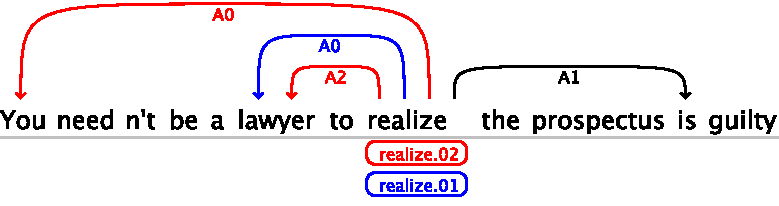
\includegraphics[scale=.58]{joint-sense-example}
% \end{center}
% \caption{Fragment of sentence in the development set that the pipeline model gets wrong: it picks the wrong sense (``02'') for ``realize'' and falsely assigns ``You'' the A0 role and ``lawyer'' the A2 role.}
% \label{fig:jointSense}
% \end{figure}


% I don't quite understand why we did isArg vs no isArg :-S. Maybe, too late to
% bring the issue. I just put two columns, if I put dev and brown, they get too
% big.
% SR: Huh? Without isArg we wouldn't need to jointly predict args for ALL predicates of one sentence. So this is to justify the joint model, and the fact that we explicitely model isArgument (different from all other SRL models I know). 

\subsection{Modelling if a Token is an Argument}
In table \ref{tbl:results} we also observe that improvements can be made if we explicitly model the decision whether a token is a semantic argument of some predicate or not. As we mentioned in section \ref{sec:model}, this aspect of our model requires us to jointly perform inference for all predicates of a sentence, and hence our results justify the per-sentence SRL approach proposed in this paper.

In order to analyse where these improvements come from, we again list our results on a per-SRL-predicate basis. Table \ref{tbl:isArg} shows that by including the $isArgument$ predicate and the corresponding formulae we gain around 0.6\% and 1.0\% points across the board for WSJ and Brown, respectively. As shown in table \ref{tbl:results}, these improvements result in about 1.0\% improvements for both WSJ and Brown in terms of the CoNLL 2008 metric. Hence, an explicit model of the ``is an argument'' decision helps the SRL at all levels \footnote{All scores in the bottom-up when compared with the version without the $isArgument$ predicate are statistically significant with exception of the $sense/2$ predicate for the Brown test set.}.

How the $isArgument$ helps to improve the overall role labelling score can be illustrated with the example in figure \ref{fig:isArg}. Here the model without a hidden $isArgument$ predicate fails to attach the preposition ``on'' to the predicate ``start.01'' (here 01 refers to the sense of the predicate). Apparently the model has not enough confidence to assign the preposition to either ``start.01'' or ``get.03'', so it just drops the argument altogether. However, because the $isArgument$ model knows that most prepositions have to be modifying some predicate, pressure is created that forces a decision between the two predicates. And because for the role model ``start.01'' looks like a better fit than ``get.03'', the correct attachment is found.

%%example
\begin{figure}
\begin{center}
    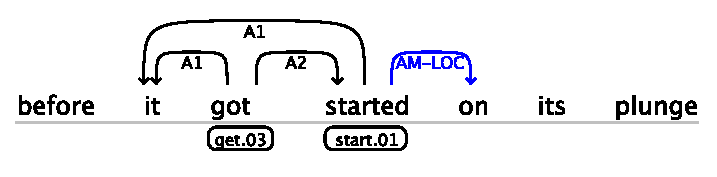
\includegraphics[scale=.62]{is-arg-example}
\end{center}
\caption{Segment of the CoNLL 2008 development set for which the bottom-up model w/o $isArgument$ predicate fails to attach the preposition ``on'' as an ``AM-LOC'' for ``started''. The joint bottom-up model attaches the preposition correctly.}
\label{fig:isArg}
\end{figure}


\begin{table}[ht]

    \centering
    \begin{tabular}{|c|c|c|c|c|}\hline
      & \multicolumn{2}{c|}{WSJ} & \multicolumn{2}{c|}{Brown}\\
                                  & w/o     & w/     & w/o    & w/  \\\hline 
        \emph{isPredicate}        & $96.3$  & $96.5$ & $91.4$ & $92.5$\\
%%        \emph{isArgument}         &         & $86.6$ &        & $86.6$ \\
        \emph{hasRole}            & $87.1$  & $87.7$ & $82.5$ & $83.6$ \\
        \emph{role}               & $76.9$  & $77.5$ & $65.2$ & $66.2$ \\
        \emph{sense}              & $88.3$  & $89.0$ & $76.1$ & $77.5$ \\\hline
    \end{tabular}
    \caption{$F_1$ scores for ML predicates; w/o refers to a Bottom-up system without isArgument predicate, w/ refers to a Bottom-up system with isArgument predicate.}
    \label{tbl:isArg}
\end{table}

% WSJ
%isPredicate, n+ 56, n- 17, p <= 5.27e-06
 %POS: 56
 %NEG: 17
%isArgument
 %POS: 10800
 %NEG: 0
%frameLabel,n+ 100, n- 50, p <= 6.31e-05
 %POS: 100
 %NEG: 50
%hasLabel, n+ 286, n- 174, p <= 2.28e-07
 %POS: 286
 %NEG: 174
%role, n+ 293, n- 196, p <= 1.42e-05
 %POS: 293
 %NEG: 196

%Brown
% isPredicate, n+ 47, n- 7, p <= 2.29e-08
% POS: 47
% NEG: 7
%isArgument
% POS: 1280
% NEG: 0
%frameLabel,n+ 21, n- 12, p <= 0.163
% POS: 21
% NEG: 12
%hasLabel, n+ 55, n- 33, p <= 0.0246
% POS: 55
% NEG: 33
%role, n+ 58, n- 32, p <= 0.00805
% POS: 58
% NEG: 32


\subsection{Efficiency}
In the previous sections we have shown that our joint model indeed does better than an equivalent pipeline system. However, usually most joint approaches come at a price: efficiency. Interestingly, in our case we observe the opposite: our joint model is actually faster than the pipeline. This can be seen in table \ref{tbl:nocpi}, where we list the time it took for several different system to process the WSJ and Brown test corpus, respectively. When we compare the times for the bottom-up model to those of the pipeline, we note that the joint model is twice as fast. While the individual stages within the pipeline may be faster than the joint system (even when we sum up inference times), extracting results from one system and feeding them into another creates overhead which offsets this potential reduction.  

Table \ref{tbl:nocpi} also lists the run-time of a bottom-up system that solves the inference problem by fully grounding the Markov Network that the Markov Logic (ML) model describes, mapping this network to an Integer Linear Program, and finding the most likely assignment using an ILP solver. This system (Bottom-up (-CPI)) is four times slower than the equivalent system that uses Cutting Plane Inference  (Bottom-up). This suggests that if we were to implement the same joint model using ILP instead of ML, our system would either be significantly slower, or we would need to implement a Cutting Plane algorithm for the corresponding ILP formulation---when we use ML this algorithm comes ``for free''. 
% \begin{table}[ht]

%     \centering
%     \begin{tabular}{|p{2.5cm}|c|c|c|}\hline
%         System                           & Training & Testing   & Testing \\
%                                          &          & WSJ       & Brown   \\\hline 
%         Full model                       & $5.1$h   & $9.2$m    & $1.5$m  \\
%         Bottom-up                        & $4.3$ih  & $9.5$m    & $1.6$m  \\
%         Full model w/o \emph{isArgument} &          &           &         \\
%         Bottom-up  w/o \emph{isArgument} & $3.9$h   & $12.5$m   & $1.5$m \\
%         Pipeline                         & $5.0$h   & $18.9$m   & $2.9$m \\\hline
%     \end{tabular}
%     \caption{Testing and training times for the systems.}
%     \label{tbl:times}
% \end{table}

\begin{table}[ht]

    \centering
    \begin{tabular}{|p{3.0cm}|c|c|}\hline
        System                           & WSJ       & Brown   \\\hline 
        Full                             & $9.2$m    & $1.5$m  \\
        Full (-CPI)                      & $38.4$m   & $7.47$m  \\
        Bottom-up                        & $9.5$m    & $1.6$m  \\
        Bottom-up (-CPI)                 & $38.8$m   & $6.9$m  \\
        Pipeline                         & $18.9$m   & $2.9$m  \\\hline
    \end{tabular}
    \caption{Testing times for full model and bottom-up when CPI algorithm is
    not used. The WSJ test set contains 2414 sentences, the Brown test set 426. Our best systems thus takes on average 230ms per WSJ sentence (on a 2.4Ghz system). }
    \label{tbl:nocpi}
\end{table}


%7. Results
%7.1 Joint/Bottom-up vs pipeline
%- Illustrate that we get dramatic improvements in sense
%disambiguation, but not in other parts. Stress effect on Brown
%- Show table that compares isPredicate & role & frameLabel results for
%pipeline vs joint models (this would show that no gain in isPredicate
%and role, but in frameLabel)
%- Give example from dev-set
%7.2 With isArg vs without isArg
%- illustrate that we get improvements in all sections
%- show table that compares individual predicate scores (dev, wsj,
%brown) for isArg vs w/o isArg
%- maybe find example?
%7.3 (Maybe) Full vs Bottom-up again (maybe not because in other paper)
%7.4 Efficiency
%- Illustrate that training the model jointly comes at no extra cost
%(we can train as fast/faster with the joint bottom up model than with
%a pipeline)
%- Illustrate that inference is much more efficient when compared to an
%equivalent ILP-only system (which is basically the w/o CPI system)
%- Can we also have a sentence/second column for testing?
%
%
%Pipeline
%**************
%         isPredicate    : 0.958,0.959,0.958,0.959,0.959
%          isArgument    : 0.890,0.892,0.891,0.891,0.891
%            hasLabel    : 0.870,0.873,0.872,0.872,0.872
%                role    : 0.706,0.718,0.720,0.722,0.723
%          frameLabel    : 0.834,0.842,0.841,0.841,0.841
%
%         isPredicate    : 0.966,0.922
%          isArgument    : 0.903,0.859
%            hasLabel    : 0.880,0.836
%                role    : 0.754,0.642
%          frameLabel    : 0.855,0.673
%
%Times :
%trainning (hrs):
%stage1= 0.76
%stage2= 3.42
%stage3= 0.84
%total = 5.02
%testing:
%stage1: 5.44m, 42.68s
%stage2: 7.56m, 1.27m 
%stage3: 5.96m, 54.03s
%total: 18.96,  2.90m
%
%
%WSJ
%  Labeled precision:          (10284 + 4521) / (13021 + 5321) * 100 = 80.72 %
%  Labeled recall:             (10284 + 4521) / (14269 + 5260) * 100 = 75.81 %
%  Labeled F1:                 78.19
%
%Brown
%  Labeled precision:          (1335 + 555) / (1986 + 846) * 100 = 66.74 %
%  Labeled recall:             (1335 + 555) / (2210 + 804) * 100 = 62.71 %
%  Labeled F1:                 64.66
%
%
%
%Full model
%**************
%         isPredicate    : 0.958,0.959,0.958,0.958,0.958
%          isArgument    : 0.894,0.895,0.895,0.895,0.895
%            hasLabel    : 0.865,0.868,0.869,0.869,0.869
%                role    : 0.703,0.713,0.720,0.724,0.727
%          frameLabel    : 0.870,0.874,0.878,0.877,0.878
%
%         isPredicate    : 0.965,0.923
%          isArgument    : 0.906,0.869
%            hasLabel    : 0.879,0.838
%                role    : 0.755,0.646
%          frameLabel    : 0.885,0.771
%
%Times:
%Training :5.09 hrs
%Testing:
%WSJ          9.15m 
%Brown        1.58m 
%
%
%WSJ
%  Labeled precision:          (10423 + 4664) / (13348 + 5273) * 100 = 81.02 %
%  Labeled recall:             (10423 + 4664) / (14269 + 5260) * 100 = 77.25 %
%  Labeled F1:                 79.09
%
%Brown
%  Labeled precision:          (1369 + 621) / (2063 + 807) * 100 = 69.34 %
%  Labeled recall:             (1369 + 621) / (2210 + 804) * 100 = 66.03 %
%  Labeled F1:                 67.64
%
%
%Full model w/o isArg (NOTE: not with new formula2/ we need it with bottom-up model as well)
%**************
%
%       isPredicate      : 0.955,0.955,0.954,0.955,0.955
%            hasLabel    : 0.860,0.863,0.866,0.865,0.865
%                role    : 0.710,0.722,0.727,0.730,0.730
%          frameLabel    : 0.869,0.874,0.875,0.876,0.875
%
%         isPredicate    : 0.963,0.910
%            hasLabel    : 0.872,0.818
%                role    : 0.752,0.638
%          frameLabel    : 0.878,0.761
%
%Times (hrs)
%Training: 4.58
%Testing:
%WSJ       9.53m 
%Brown     1.43m 
%
%
%
%WSJ
%  Labeled precision:          (10308 + 4615) / (13132 + 5257) * 100 = 81.15 %
%  Labeled recall:             (10308 + 4615) / (14269 + 5260) * 100 = 76.41 %
%  Labeled F1:                 78.71
%
%Brown
%  Labeled precision:          (1324 + 609) / (1973 + 797) * 100 = 69.78 %
%  Labeled recall:             (1324 + 609) / (2210 + 804) * 100 = 64.13 %
%  Labeled F1:                 66.84
%
%
%
%Bottom up
%**************
%         isPredicate    : 0.958,0.960,0.960,0.960,0.959
%          isArgument    : 0.893,0.895,0.895,0.894,0.894
%            hasLabel    : 0.867,0.870,0.869,0.870,0.869
%                role    : 0.728,0.738,0.743,0.746,0.747
%          frameLabel    : 0.872,0.878,0.885,0.887,0.883
%
%         isPredicate    : 0.965,0.925
%          isArgument    : 0.904,0.866
%            hasLabel    : 0.877,0.836
%                role    : 0.775,0.662
%          frameLabel    : 0.890,0.775
%
%Times:
%Training 4.26 hrs
%Testing:
%WSJ          9.53m 
%Brown        1.55m 
%
%WSJ
%  Labeled precision:          (10315 + 4590) / (12349 + 5262) * 100 = 84.63 %
%  Labeled recall:             (10315 + 4590) / (14269 + 5260) * 100 = 76.32 %
%  Labeled F1:                 80.26
%
%Brown
%  Labeled precision:          (1327 + 591) / (1836 + 812) * 100 = 72.43 %
%  Labeled recall:             (1327 + 591) / (2210 + 804) * 100 = 63.64 %
%  Labeled F1:                 67.75
%
%
%NO CPI 
%**************
%         isPredicate    : 0.959,0.958,0.958,0.957,0.957
%          isArgument    : 0.894,0.896,0.895,0.895,0.893
%            hasLabel    : 0.867,0.869,0.870,0.868,0.867
%                role    : 0.708,0.720,0.726,0.727,0.727
%          frameLabel    : 0.873,0.878,0.880,0.879,0.879
%
%         isPredicate    : 0.964,0.925
%          isArgument    : 0.905,0.865
%            hasLabel    : 0.877,0.836
%                role    : 0.775,0.661
%          frameLabel    : 0.886,0.778
%
%Times:
%training: 6.51 hrs
%testing:
% WSJ        38.06m
% Brown       6.73m 
%
%WSJ     
%  Labeled precision:          (10323 + 4546) / (12384 + 5267) * 100 = 84.24 %
%  Labeled recall:             (10323 + 4546) / (14269 + 5260) * 100 = 76.14 %
%  Labeled F1:                 79.98
%
%Brown
%  Labeled precision:          (1324 + 600) / (1833 + 812) * 100 = 72.74 %
%  Labeled recall:             (1324 + 600) / (2210 + 804) * 100 = 63.84 %
%  Labeled F1:                 68.00
%
%
%Without linguistic
%**************
%
%
%
%
%bottom-up w/o isArg
%**************
%         isPredicate    : 0.953,0.955,0.955,0.955,0.954
%            hasLabel    : 0.859,0.863,0.863,0.863,0.862
%                role    : 0.725,0.739,0.742,0.743,0.745
%          frameLabel    : 0.870,0.875,0.877,0.876,0.876
%
%         isPredicate    : 0.963,0.914
%            hasLabel    : 0.871,0.825
%                role    : 0.769,0.652
%          frameLabel    : 0.883,0.761
%
%Times
%Training: 3.84 hrs
%Testing:
%WSJ         12.52m
%Brown        1.50m 
%
%WSJ
%  SEMANTIC SCORES:
%  Labeled precision:          (10218 + 4495) / (12293 + 5252) * 100 = 83.86 %
%  Labeled recall:             (10218 + 4495) / (14269 + 5260) * 100 = 75.34 %
%  Labeled F1:                 79.37
%
%
%Brown
%  Labeled precision:          (1298 + 578) / (1806 + 805) * 100 = 71.85 %
%  Labeled recall:             (1298 + 578) / (2210 + 804) * 100 = 62.24 %
%  Labeled F1:                 66.70
%
%





%\subsection{Analysis}\label{sec:analysis}


%%% Local Variables: 
%%% mode: latex
%%% TeX-master: "paper"
%%% End: 

%There are two particular types of errors our system produces. First, errors that assing seemingly random ``R-AA'' label to token pairs. And second, errors on nominal predicates. 

A substantial amount of errors in our submitted results~(Full) can be attributed to the seemingly random assignment of the very low frequency label ``R-AA'' (appears once in the training set) to token pairs that should either have a different role or no role at all. Without these false positives precision would increase by about 1\%. Interestingly, this type of error completely disappears for the bottom-up model~(Up) and thus seem to be crucial in order understand why this model can outperform the full model. 

We believe that this type of error is an artifact of the training regime. For the full model the weights of the \emph{role} predicate only have ensure that the right (true positive) role is the relative winner among all roles. In the bottom-up model they also have to make sure that their cumulative weight is nonnegative -- otherwise simply not assigning a role $r$ for $(p,a)$ would increase the score even if \emph{hasRole(p,a)} is predicted with high confidence. Thus more weight is shifted towards the proper roles. This helps the right label to win more likely over the ``R-AA'' label, whose weights have rarely been touched and are closer to zero.

Likewise, in the bottom-up model the total weight of the \emph{hasRole} features of a wrong (false positive) candidate token pair must be nonpositive. Otherwise picking the wrong candidate would increase overall score and no \emph{role} features can reject this decision because the corresponding structural constraints are missing. Thus more weight is shifted away from false positive candidates, resulting in a higher precision of the \emph{hasRole} predicate. This also means that less wrong candidates are proposed, for which a ``R-AA'' role is more likely to be picked because its weights have hardly been touched.

% In our results of joint model for the development set the label ``R-AA'' (meaning a reference to an AA argument) was assigned 351 times. However, the gold data does not contain this label at all and thus this behaviour amounts to a HOWMUCH loss of precision. This error happens in cases where a label has to be assigned to a token pair in context that is substantially different from those seen in the training set\footnote{For example, when the \emph{hasLabel} requires a label for the pair $(p,a)$ and $p$ is not even a predicate.} and for which only very general high frequency features are active. 

% To explain this behaviour let us consider that roles have low and high frequency roles (such as ``A1'' and ``R-AA'') and features (such as lexicalised and POS tag features). During online learning the current model will sometimes wrongly predict a high frequency role instead of another high frequency role(for example because in certain cases ``A1'' and ``A2'' labels can be confused). In these cases the features weights for this role label are decreased. However, we will hardly ever predict ``R-AA'' instead of a high frequency role such as ``A1'' because there will be certain features that support ``A1''. Thus the weights for the low frequency role ``R-AA'' are decreased less likely. 

% Likewise, in the top-down pipeline the weights of the \emph{hasLabel} features need to ensure that by classifying a wrong token pair as candidate the overall score is not increased -- otherwise classifying it as candidate improves the solution. Again, for the joint model this does not hold: even if the contribution of the \emph{hasLabel} features might increase the score, the \emph{role} features can penalise this decision by penalising all possible roles. Thus (high frequency) features appearing in false positives candidates have less weight, causing higher precision for the \emph{hasLabel} predicate. 

% When we encounter a context with many low frequency features then it is likely that most of their weights are untouched and still at zero. What remains are the high frequency features. In the case of high frequency roles the weights of these features have been decreased often. However, for low-frequency roles the high frequency feature weights weren't touched that often. Thus we observe that these weights are larger than those of the high frequency roles. This results in a low frequency roles predicted in a unknown context.

% Interestingly, this type of error is completely avoided when using the ``top-down-pipeline'' discussed above -- the label ``R-AA'' is not assigned at all. During the training of this model it is not enough for low frequency features to make their corresponding role label the \emph{relative} winner among all roles. They must also ensure that by assigning their label the global solution does not loose score -- otherwise simply not assigning a role always improves the solution. In the case of the joint model this does not hold: while the features of each role might reduce the score of the global solution removing them would also remove the corresponding hasLabel decision, which could reduce the score more dramatically. Thus low frequency features will have more weight and produce higher precision in unlikely contexts. 

% Likewise, in the top-down pipeline the weights of the \emph{hasLabel} features need to ensure that by classifying a wrong token pair as candidate the overall score is not increased -- otherwise classifying it as candidate improves the solution. Again, for the joint model this does not hold: even if the contribution of the \emph{hasLabel} features might increase the score, the \emph{role} features can penalise this decision by penalising all possible roles. Thus (high frequency) features appearing in false positives candidates have less weight, causing higher precision for the \emph{hasLabel} predicate. 

Another prominent type of errors appear for nominal predicates. Our system only recovers only about 80\% of predicates with ``NN'', ``NNS'' and ``NNP'' tags (and classifies about 90\% of these with the right predicate sense). Argument identification and classification performs equally bad. For example, for the ``A0'' argument of ``VB'' predicates we get an F-score of 82.00\%. For the ``A0'' of ``NN'' predicates F-score is 65.92\%. The features of our system are essentially taken from the work done on PropBank predicates and we did only little work to adapt these to the case of nominal predicates. Putting more effort into designing features specific to the case of nominal predicates might improve this situation.


% More importantly, the top-down pipeline also shifts more weight from the wrong \emph{hasLabel} decisions because when the \emph{hasLabel} formulas predict a false positive the \emph{role} formulas cannot overrule this to make the decision right. 

% Model 1: 
%   - role has to be relative winner
%   - hasLabel 
% Model 3: 
%   - role has to be relative winner and must not decrease score (delta s > 0)
%   - hasLabel (classifies 

% We believe that this is because during training 

% Model 3 shifts weight more often on the true \emph{role} labels because even though the \emph{hasLabel} predicate predicts the existence of a label the \emph{role} predicate is not required to pick one an will make a mistake even the score of the right label is not high enough even though its relative score is higher than the rest. It also shifts more weight from the wrong \emph{hasLabel} decisions because when the \emph{hasLabel} formulas predict a false positive the \emph{role} formulas cannot overrule this to make the decision right. 

% In the course of MIRA online learning the high frequency roles are sometimes incorrectly assigned to token pair candidates. In these cases the weights of high frequency features of these roles are decreased. 

%  for which no or very few features fire. For example, this is the case if the \emph{isPredicate} and \emph{hasLabel} features predict a token pair to be labelled even though the proposed predicate is a preposition. In this case only very general features compete against each other; however while the general weights for high frequency roles have been touched during training whenever for every false positive that appears during online learning, the general weights for low frequency roles did not come up as often because false positive ``R-AA'' scores are usually outscored by the true positive scores of the right labels. Thus ``R-AA'' is likely to have a higher score than the high frequency/more likely labels in such contexts. 






\section{Conclusion} \label{sec:conclusion}



We presented a Markov Logic Network that performs joint multi-lingual Semantic 
Role Labelling. This network achieves the third best semantic F-scores in the 
closed track among the SRLOnly systems of the CoNLL-09 Shared Task, and sixth 
best semantic scores among SRLOnly and Joint systems for the closed task.
% SR closed or open???

We observed that the inclusion of features which take into account 
information about the siblings of the argument were beneficial for 
SRL performance on the Japanese dataset. We also noticed that our poor performance with Czech 
are caused by our frame ID heuristic. Further work 
has to be done in order to overcome this problem. 


\bibliographystyle{plainnat}
\bibliography{extra,seb}

\end{document}

% Reviwer 1

% 1. native speaker
% 2. Remove 4.1 subheading (done! take out the reference to the label as well )
% 3. Include average scores (done)
% 4. Table 1 reference wrong render (done)
% 5. Fix footnotes (done).
% 6. Use \noindent in the list 
% 7. Typos
    %Abstract:
    %"Task in" -> "Task on" (done)
    %"focus only in" -> "focus only on" (done)
    %"closed Track for SRLOnly system" -> "closed track for SRLOnly systems" (done)
    %Page 1:
    %"that require to answer ... questions" -> "that are required to answer
    %questions such as ..." (done)
    %Page 2:
    %"refer predicates" -> "refer to predicates" (done)
    %The third item in the list is not syntactically coherent. (kind of done)
    %Page 3:
    %"The here presented ML predicates" -> "The ML predicates presented here" (done)
    %Page 4:
    %"these lists does" -> "these lists do" (done)
    %The caption of Table 1 is garbled. (done)
    %Page 5:
    %"empiricaly" -> "empirically" (not found)
    %"SRLonly-closed track" -> "closed track for SRLOnly systems" (not found)
    %"f1" -> "F1" (done)
    %"for the English" -> "for English" (done)
    %"of rather technical" -> "of a rather technical" (done)

% Reviewer 2.
% Minor issues:
% p1. the last sentence in abstract: => .. sixth for joint systems. (done)
% p4. right column, the reference to Table 1 is broken and shown as ?? 


% Our notes:
%   * Change descripions of rules for shorter versions (use templates, maybe put them into tables with smaller font size—-the bullet points don't look to good I think)
%   * Clarify the use of modules
%   * Fix Czech sense heuristic?
%   * Show some numbers that explain check problems?
%   * Explain effect of Japanese formulae
 
